\documentclass[sigconf, nonacm]{acmart}
\usepackage{pdfpages}
\usepackage{amsmath}
\usepackage{listings}
\usepackage{titlesec}
\setcounter{secnumdepth}{5}
\newcommand*\textfrac[2]{
  \frac{\text{#1}}{\text{#2}}
}
\newcommand{\RefFig}[1]{\textit{~\ref{#1} on page ~\pageref{#1}}}




\usepackage{color}
\definecolor{lightgray}{rgb}{.9,.9,.9}
\definecolor{darkgray}{rgb}{.4,.4,.4}
\definecolor{purple}{rgb}{0.65, 0.12, 0.82}
\definecolor{green}{rgb}{.2, .8, 0}
\lstdefinelanguage{JavaScript}{
  keywords={=>, break, case, catch, continue, debugger, default, delete, do, else, false, finally, for, function, if, in, instanceof, new, null, return, switch, this, throw, true, try, typeof, var, void, while, with},
  morecomment=[l]{//},
  morecomment=[s]{/*}{*/},
  morestring=[b]',
  morestring=[b]",
  morestring=[b]`,
  ndkeywords={const, class, export, boolean, throw, implements, import, this},
  keywordstyle=\color{blue}\bfseries,
  ndkeywordstyle=\color{blue}\bfseries,
  identifierstyle=\color{black},
  commentstyle=\color{purple}\ttfamily,
  stringstyle=\color{green}\ttfamily,
  sensitive=true
}

\lstset{
   language=JavaScript,
   backgroundcolor=\color{lightgray},
   extendedchars=true,
   basicstyle=\footnotesize\ttfamily,
   showstringspaces=false,
   showspaces=false,
   numbers=left,
   numberstyle=\footnotesize,
   numbersep=9pt,
   tabsize=2,
   breaklines=true,
   showtabs=false,
   captionpos=b
}
\lstdefinelanguage{HTML5}{
        language=html,
        sensitive=true, 
        alsoletter={<>=-},
        otherkeywords={
        % HTML tags
        <html>, <head>, <title>, </title>, <meta, />, </head>, <body>,
        <canvas, \/canvas>, <script>, </script>, </body>, </html>, <!, html>, <style>, </style>, ><
        },  
        ndkeywords={
        % General
        =,
        % HTML attributes
        charset=, id=, width=, height=,
        % CSS properties
        border:, transform:, -moz-transform:, transition-duration:, transition-property:, transition-timing-function:
        },  
        morecomment=[s]{<!--}{-->},
        tag=[s]
}
%% complete the rights form.
\setcopyright{none}

%% These commands are for a PROCEEDINGS abstract or paper.
\acmConference[Dundee Computing Honours Project '22]{Computing Honours Projects '22: The University of Dundee Computing Project Showcase: '22.}{2022}{Dundee, UK}


%%
%% end of the preamble, start of the body of the document source.
\begin{document}

%%
%% The "title" command has an optional parameter,
%% allowing the author to define a "short title" to be used in page headers.
\title{Code Quality Analysis}


\author{Christy McCarron}
\email{cswmccarron@dundee.ac.uk}
\affiliation{%
  \institution{University of Dundee}
  \city{Dundee}
  \state{Scotland}
  \country{UK}
}

%%
%% The abstract is a short summary of the work to be presented in the
%% article.

\begin{abstract}
Your abstract will go here.
\end{abstract}


%% A "teaser" image appears between the author and affiliation
%% information and the body of the document, and typically spans the
%% page.
\begin{teaserfigure}
  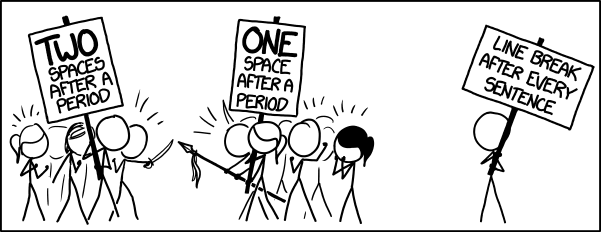
\includegraphics[width=\textwidth]{images/third_way.png}
  \caption{Third Way, xkcd}
  \Description{xkcd comic on language choices}
  \label{fig:thirdWay}
\end{teaserfigure}

%%
%% This command processes the author and affiliation and title
%% information and builds the first part of the formatted document.
\maketitle


% THIS IS THE MAIN PARTS OF THE DOCUMENT
\section{Introduction}
Code quality can be subjective, each person and organisation will have differing needs and wants when it comes to the quality of their code. But there are a many well defined areas that are as universal as can be.

test test
1234 aaa bbbb
\subsection{Secondary Part}
This is \textbf{another} part of my \textit{introduction}.

\begin{enumerate}
    \item This is the first item
    \item This is the second item
\end{enumerate}

This is another line of text that will go here

\begin{itemize}
  \item List entries start with the \verb|\item| command.
  \item Individual entries are indicated with a black dot, a so-called bullet.
  \item The text in the entries may be of any length.
\end{itemize}

\begin{table}[h]
\begin{tabular}{lll}
\hline
Colour & Score & Rating \\ \hline
Red    & 5     & B+     \\
Green  & 8     & A      \\ \hline
\end{tabular}
\end{table}
\section{Background}
In this project the student will focus on Static Analysis methods which are performed on source code this is as opposed to Dynamic Analysis which involves running the program and evaluating the quality while stepping through execution.

There are many ways to measure code quality but what we must establish is:
\begin{itemize}
    \item The code must do what it is meant to do.
    \item The code must be able to be tested.
    \item The code must be well documented.
    \item The code is readable and understandable.
    \item The code must be extendable.
\end{itemize}
\subsection{Tokenizing}
\begin{figure}[h]
    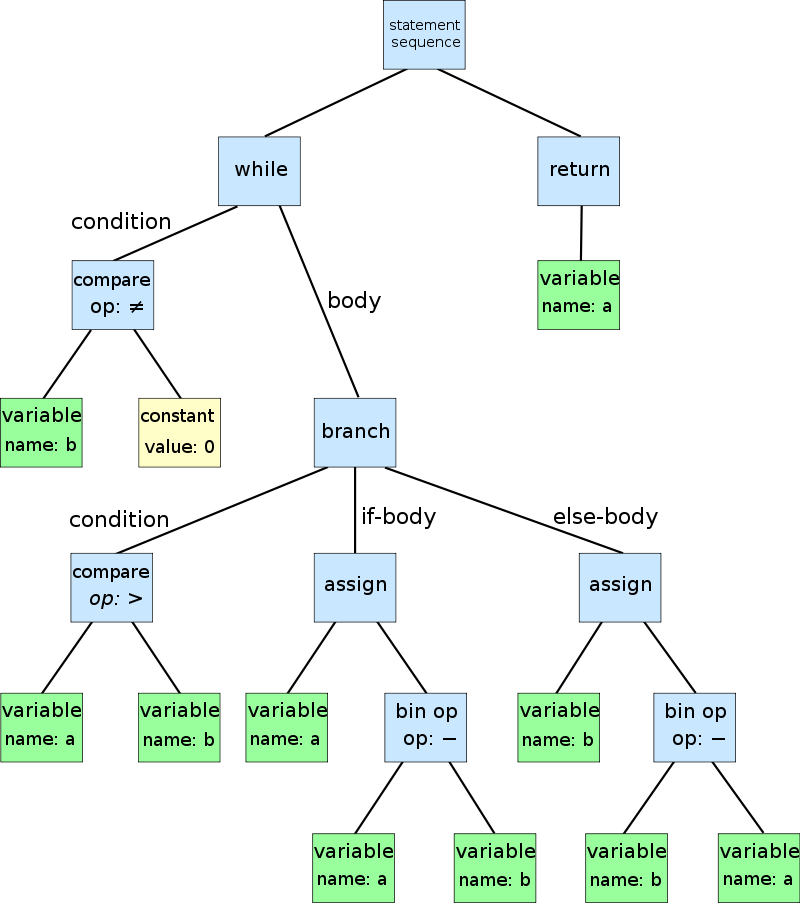
\includegraphics[width=.2\textwidth]{images/abstract-syntax-tree.png}
    \caption{Abstract Syntax Tree}
    \Description{graphical representation of abs of euclid algorithm}
    \label{fig:abs}
\end{figure}
In order to create a representation of the code we must tokenize the source code into it's component pieces and store this in an Abstract Syntax Tree. We can then use this representation of the code to preform our analysis.
The below code has been transformed into the AST in Figure.
\begin{verbatim}
    while b != 0
    if a > b
       a := a - b
    else
        b := b - a
    return a
\end{verbatim}
Each possibility in execution is converted to a tree which follows the path.
\subsection{Complexity Measures}
To measure code complexity there are a number of algorithms which measure different aspects of complexity of the code. These measure are agnostic to the language used so once the source code has been converted to an Abstract Syntax Tree any language may be evauluated by them.
\subsubsection{Halstead Complexity Measures}
In his 1977 book M.H. Halstead described a set of complexity measures. \cite{HalsteadComplexity}
\newline
These are described as such for any software program.
\begin{itemize}
    \item n\textsuperscript{1} : the number of unique operators
    \item n\textsuperscript{2} : the number of unique operands
    \item N\textsuperscript{1} : the total number of operators
    \item N\textsuperscript{2} : the total number of operands
\end{itemize}
Then several measures can be calculated from these.
\begin{itemize}
    \item Program Vocabulary    : n = n\textsuperscript{1} + n\textsuperscript{2}
    \item Program length        : N = N\textsuperscript{1} + N\textsuperscript{2}
    \item Calculated estimated program length : \^{N} = n\textsuperscript{1} log \textsubscript{2} n\textsuperscript{1} + n\textsuperscript{2} log \textsubscript{2} n\textsuperscript{2}
    \item Volume                : V = N * log \textsubscript{2} n
    \item Difficulty            : D =  $\textfrac{n\textsuperscript{1}}{2}$ * $\textfrac{N\textsuperscript{1}}{n\textsuperscript{1}}$
    \item Effort                : D * V
    \item Time required to program : T = $\textfrac{E}{18}$
    \item Number of delivered bugs : B = $\textfrac{V}{3000}$
\end{itemize}

\begin{verbatim}
    main()
    {
        int a, b, c, avg;
        scanf("%d %d %d", &a, &b, &c);
        avg = (a+b+c)/3;
        printf("avg = %d", avg);
    }
\end{verbatim}
In this example c program 
\begin{itemize}
    \item n\textsuperscript{1} : 12
    \item n\textsuperscript{2} : 7
    \item n : 19
    \item N\textsuperscript{1} : 27
    \item N\textsuperscript{2} : 15
    \item N : 42
    \item \^{N} : 12 log \textsubscript{2} 12 + 7 log \textsubscript{2} 7 = 62.67
    \item V : 42 * log \textsubscript{2} 19 = 178.4
    \item D : $\textfrac{12}{2}$ * $\textfrac{15}{7}$ = 12.85
    \item E : 12.85 * 178.4 = 2292.44
    \item T : $\textfrac{2292.44}{18}$ = 127.357 seconds
    \item B : $\textfrac{178.4}{3000}$ = 0.059
\end{itemize}

\subsubsection{Cyclomatic Complexity}
Cyclomatic Complexity(CC) is defined as 
\begin{verbatim}
    The number of linearly independant paths within a piece of code
\end{verbatim}
For example 
\newline
This piece of code has a CC of 1

\begin{verbatim}
    function test(a){
        return a
    }
\end{verbatim}
So does this
\begin{verbatim}
    function test(a){
        let b = a
        b = a*b
        b*=42
        return b
    }
\end{verbatim}
But when we add a control statement with 2 paths our control flow graph now contains 2 possible flows which gives us a CC of 2
\begin{verbatim}
    function test(a){
        if(a>2){
            return a
        }
        return b
    }
\end{verbatim}

This is an excellent measure to follow as not only does it make us segment our code for readability and extendability it ensures there are not too many test cases for a function.
\newline
McCabe suggested this in his 1976 paper \cite{cycloMaticComplexity}
\begin{verbatim}
    "Programmers have been required to calculate complexity as 
    they create software modules. When the complexity exceeded 
    10 they had to either recognize and modularize subfunctions 
    or redo the software. The intention was to keep the "size" 
    of the modules manageable and allow for testing all the 
    independent paths..."
\end{verbatim}
    
\section{Methodology}
\subsection{\textbf{Project Management}}
\begin{figure}
    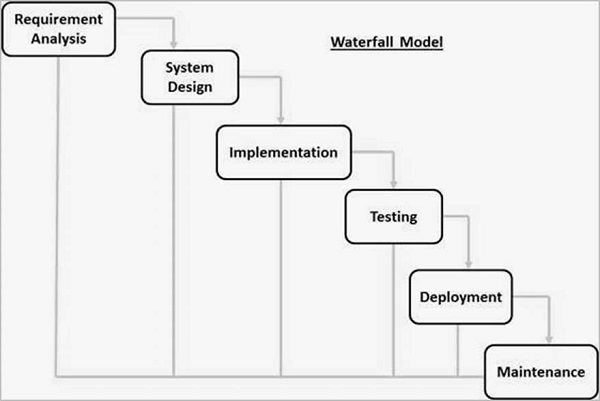
\includegraphics[width=.3\textwidth]{images/sdlc_waterfall_model.jpg}
    \caption{Flow graph showing steps of waterfall method \cite{waterfallimage}}
    \Description{Flow graph showing steps of waterfall method}
    \label{fig:waterfall}
\end{figure}
When choosing methodologies the student had 2 choices, to use a traditional software management technique such as Waterfall or a more modern approach such as Agile.
Waterfall is as described by Dr. Winston W. Royce \cite{waterfall} and as shown in Figure \RefFig{fig:waterfall}.
To be a management strategy in which the stages are quite rigid and unchanging, best suited to a project that is less likely to have changes during the development process
as the subject area being explored was new to the student, it was going to be likely to see change within requirements. The creation of
an artifact for end users and the communication with them during the process.
Whereas Waterfall is a rigid methodology thriving on predefined requirements Agile, as described in The Agile Manifesto
\cite{agile} allows for constantly changing requirements, adapting to the needs of the project and the end user and often working better
for smaller projects \cite{waterfallvsagile}.
\begin{figure}
    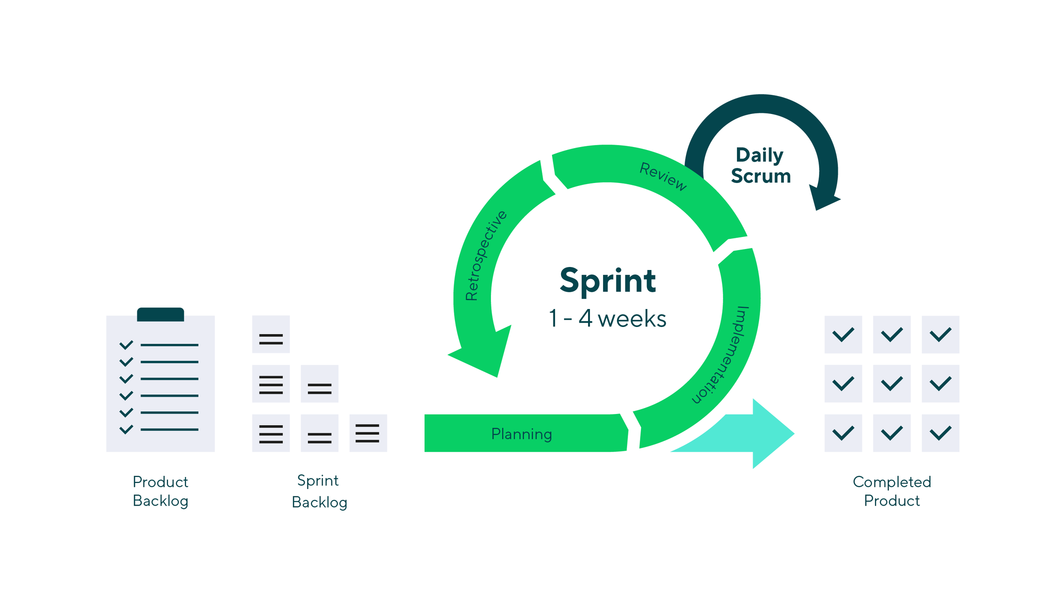
\includegraphics[width=.4\textwidth]{images/scrum-cycle-resized.png}
    \caption{Steps of a sprint \cite{sprints}}
    \Description{Steps of a sprint}
    \label{fig:sprints}
\end{figure}
With this information in mind, the student took the approach of implementing agile with 2 week long sprints \RefFig{fig:sprints}.
\begin{figure}
    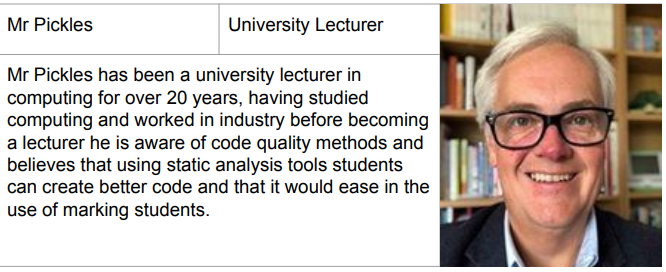
\includegraphics[width=.3\textwidth]{images/user-personas.png}
    \caption{Lecturer User Persona, see appendix D}
    \Description{Lecturer User Persona}
    \label{fig:userpersona}
\end{figure}
\subsubsection{\textbf{Creation of User Personas}}
User personas are an idea of a stereotypical user within a system. The student created 3 user stories to help better understand the end users of the system, these include
Lecturer, Developer and Student. See an example in Figure \RefFig{fig:userpersona} See Appendix D.

\subsubsection{\textbf{Creation of User Stories}}
User Stories were created with the User Personas in mind. User Stories are a clear and brief description of functionality that valuable to end users \cite{userStories}.
\begin{figure}
    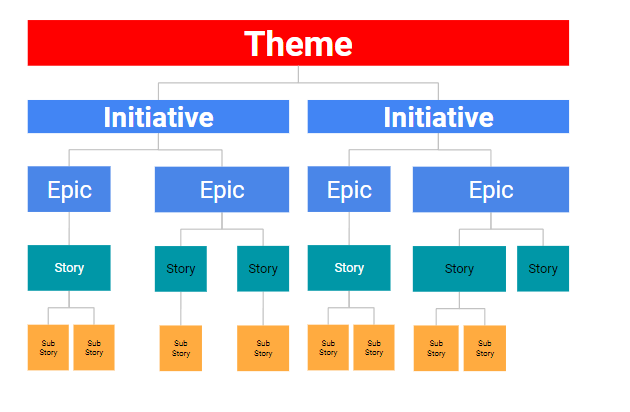
\includegraphics[width=.5\textwidth]{images/user-stories-structure.png}
    \caption{Structure of User Stories, See Appendix E}
    \Description{Structure of User Stories}
    \label{fig:userstorytheme}
\end{figure}
\begin{figure}
    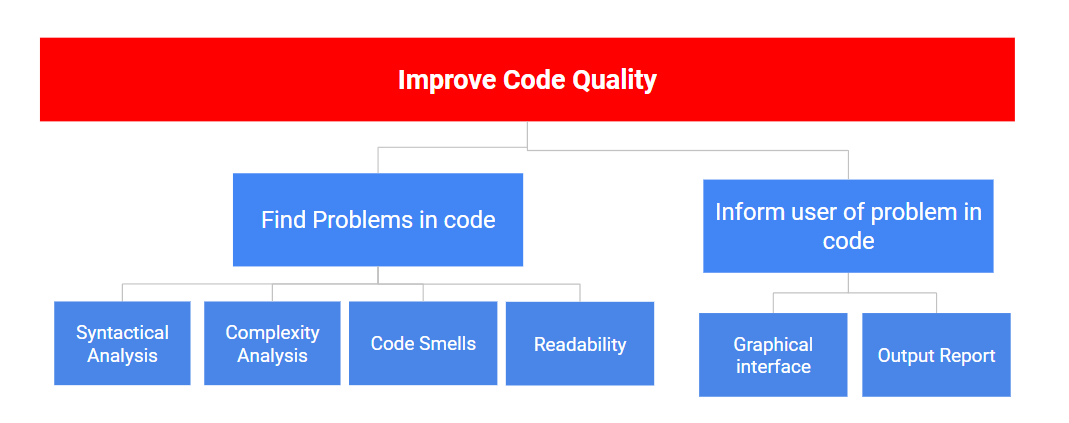
\includegraphics[width=.5\textwidth]{images/user-stories-structure-filled.png}
    \caption{User Stories Theme, Initiatives and Epics, See Appendix E}
    \Description{User Stories Theme, Initiatives and Epics, See Appendix E}
    \label{fig:userstories}
\end{figure}
Within the process of creating User Stories, a structure was created as shown in Figure \RefFig{fig:userstorytheme} and Figure \RefFig{fig:userstories}.
A theme is the Overall idea of what we are trying to create, in a larger organisation or project there could be multiple themes although as the project is limited in 
scope there is only one theme, the student felt it was prudent to ensure that the overall goal for the project to be instantiated.
An Initiative is downstream from the Theme, it is something that we want to achieve and it's Epics will again be lower level ideas of how to 
achieve this. Within an epic we finally have our user stories which describe a goal from the perspective of a user. Each User Story may have Sub Stories which take a 
more granular look at the component parts to complete that User Story , an example is Figure \RefFig{fig:complexity-userstory}
\begin{figure}
    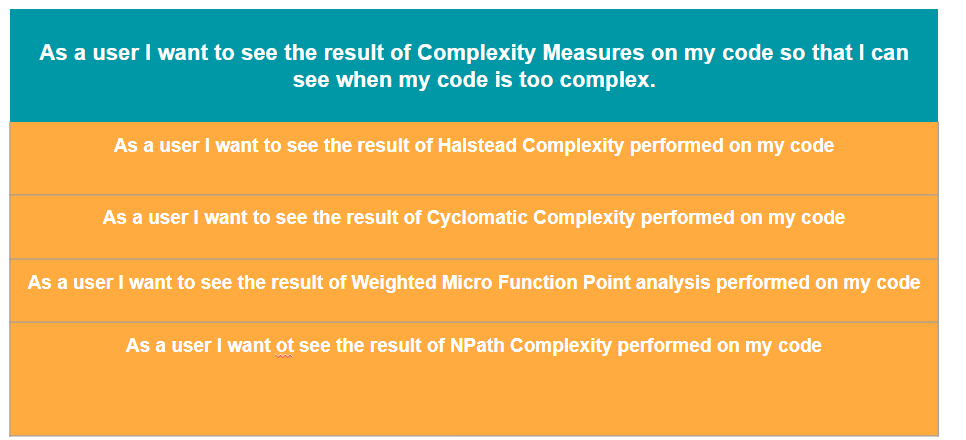
\includegraphics[width=.5\textwidth]{images/user-stories-example.png}
    \caption{Complexity Analysis User Story, See Appendix E}
    \Description{Complexity Analysis User Story, See Appendix E}
    \label{fig:complexity-userstory}
\end{figure}
\begin{figure}
    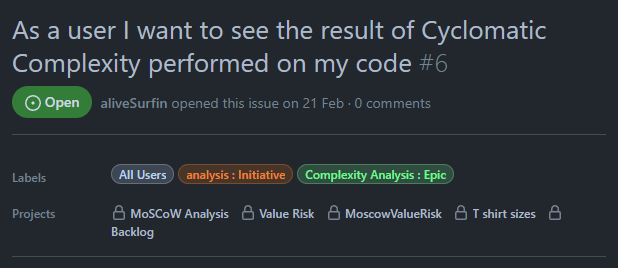
\includegraphics[width=.5\textwidth]{images/github-issue.png}
    \caption{User Story as Github Issue, See Appendix F}
    \Description{User Story as Github Issue, See Appendix F}
    \label{fig:github-issue}
\end{figure}
\subsubsection{\textbf{User Story Prioritisation and Estimation}}
User Stories were then converted to Github Issues for ease of tracking see Figure \RefFig{fig:github-issue}.
\newline
Using the Project Boards the issues were Prioritised and Estimated using a number of different methods.
The first of which is MoSCoW analysis which is a prioritisation technique in which the story is categorised into 4 distinct groups.

\begin{itemize}
    \item \textbf{MUST} - Must have this item
    \item \textbf{SHOULD} - Should complete this item if it is possible
    \item \textbf{COULD} - Could have this item if it is possible
    \item \textbf{WON'T} - Won't have this item, but would be nice to have in the future.
\end{itemize}
\cite{moscow}
User stories were separated into their distinct categories, see Appendix G.
\newline
The next method of prioritisation was Value/Risk analysis.
\begin{itemize}
    \item \textbf{Value} - How much value will completing this story item deliver to the created user personas.
    \item \textbf{Risk} - How difficult will it be to implement, will it take a long time to learn the skills associated and implement the feature. Will it have a high risk of failure?
\end{itemize}
These are then slotted into a matrix of 4 sections
\begin{itemize}
    \item \textbf{High Value - Low Risk} - These are the priority story points as they are the easiest to complete and provide the most value to users.
    \item \textbf{High Value - High Risk} - Less priority than above but still important as they provide high value to users.
    \item \textbf{Low Value - Low Risk} - Nice to have , only completed when downtime in the project.
    \item \textbf{Low Value - High Risk} - Unless there is massive downtime in development or the Risk value changes there is usually not a reason to implement this features
\end{itemize}
User Stories were separated into a Value/Risk board , see Appendix H.
\newline
These two prioritisation methods are combined to create a final priority board. This created these final sections. See appendix I.
\begin{enumerate}
    \item \textbf{High Low - Must}
    \item \textbf{High High - Must}
    \item \textbf{High Low - Should}
    \item \textbf{High High - Could}
    \item \textbf{Low Low - Could}
    \item \textbf{High High - Should}
    \item \textbf{Low High - Won't}
    \item \textbf{Low High - Could}
\end{enumerate}
These priorities would be used to determine the backlog for the project and sprints.
\newline
The final technique used was an estimation technique known as T-Shirt Sizing. Stories are estimated to be of the following sizes.
\begin{itemize}
    \item \textbf{XS}
    \item \textbf{S}
    \item \textbf{M}
    \item \textbf{L}
    \item \textbf{XL}
\end{itemize}
The first story was slotted into M and then subsequent tasks were 
added to the board in relation to the first task, this allowed the student to easier allocate based on bigger or smaller. See Appendix J.

\subsection{Test Driven Development}
For the backend coding, a Test Driven Development approach was taken, this involves writing the tests for a piece of software before you write the software 
this is said to increase code quality and also creates a cleaner design, by forcing the developer to envision the end function while writing the tests as shown in Figure 
\RefFig{fig:example-test} \cite{tdd}.
\newline
The student found this held true as although a test driven development approach was taken, a few parts of the software was written without a test in mind and these 
always turned to be less well designed and more likely to develop bugs.
\begin{figure}
    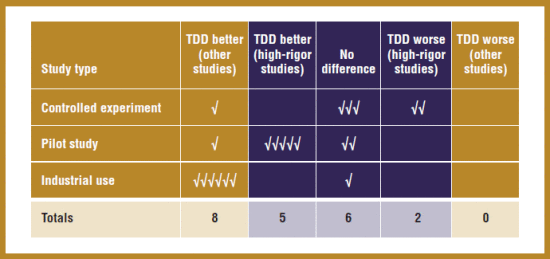
\includegraphics[width=.4\textwidth]{images/tdd effect.png}
    \caption{Effect of tdd on software outcomes \cite{tdd}}
    \Description{Effect of tdd on software outcomes}
    \label{fig:tdd}
\end{figure}
\begin{figure}[h]
\begin{lstlisting}[language=Javascript]
import Parser from "../Parser"
// table of tests [program,expectedOutput]
const testTable = [
    [``, {
        "type": "Program",
        "body": []
    }]        
]
        
const parser = new Parser()
describe('Testing empty program ', () => {
    describe.each(testTable)('parsing %s', ((program, expected) => {
        
        test(`returns ${JSON.stringify(expected)}`, () => {
            expect(parser.parse(program)).toEqual(expected)
        })
    }))
})
\end{lstlisting}
    \caption{Empty Program Parser test from "/parsing/parser/tests/empty-program.test.js" See Appendix K}
    \Description{Empty Program Parser test from "/parsing/parser/tests/empty-program.test.js" See Appendix K}
    \label{fig:example-test}
\end{figure}

\subsection{Summary}
In summary the student decided to use an agile management method, utilising stories and a backlog to ensure development. As well as using test driven development to ensure 
the quality of their software.
\section{Development}
The main features of the project are as follows
\begin{itemize}
    \item Web Interface with pseudo code editor
    \item Panel to control what analysis to perform
    \item Report Output
    \item Complexity analysis
    \item Syntactical analysis
    \item Code Smell Checking
    \item Readability checking
\end{itemize}

These items are also described in the User Stories Appendix

The student decided on using a node stack for the application, with a front end written in react fetching results from a node api.
\newline
This was chosen as it would allow for seemless use of commandline and web interface use of the program.


Sprints explainer

Sprint x 

items planned for sprint

day by day development

changes due to user testing

\newpage
\newpage
\section{Description of the final product}
The final project is hosted at \href{https://code-quality-honours.herokuapp.com/}{https://code-quality-honours.herokuapp.com/} See Appendix U.
\newline
\textbf{Overall Product}
\newline
In Figure \RefFig{fig:finalproduct} we can see a screenshot of the final product, the code editor on the left and the analysis output on the right.
\begin{figure}[h]
    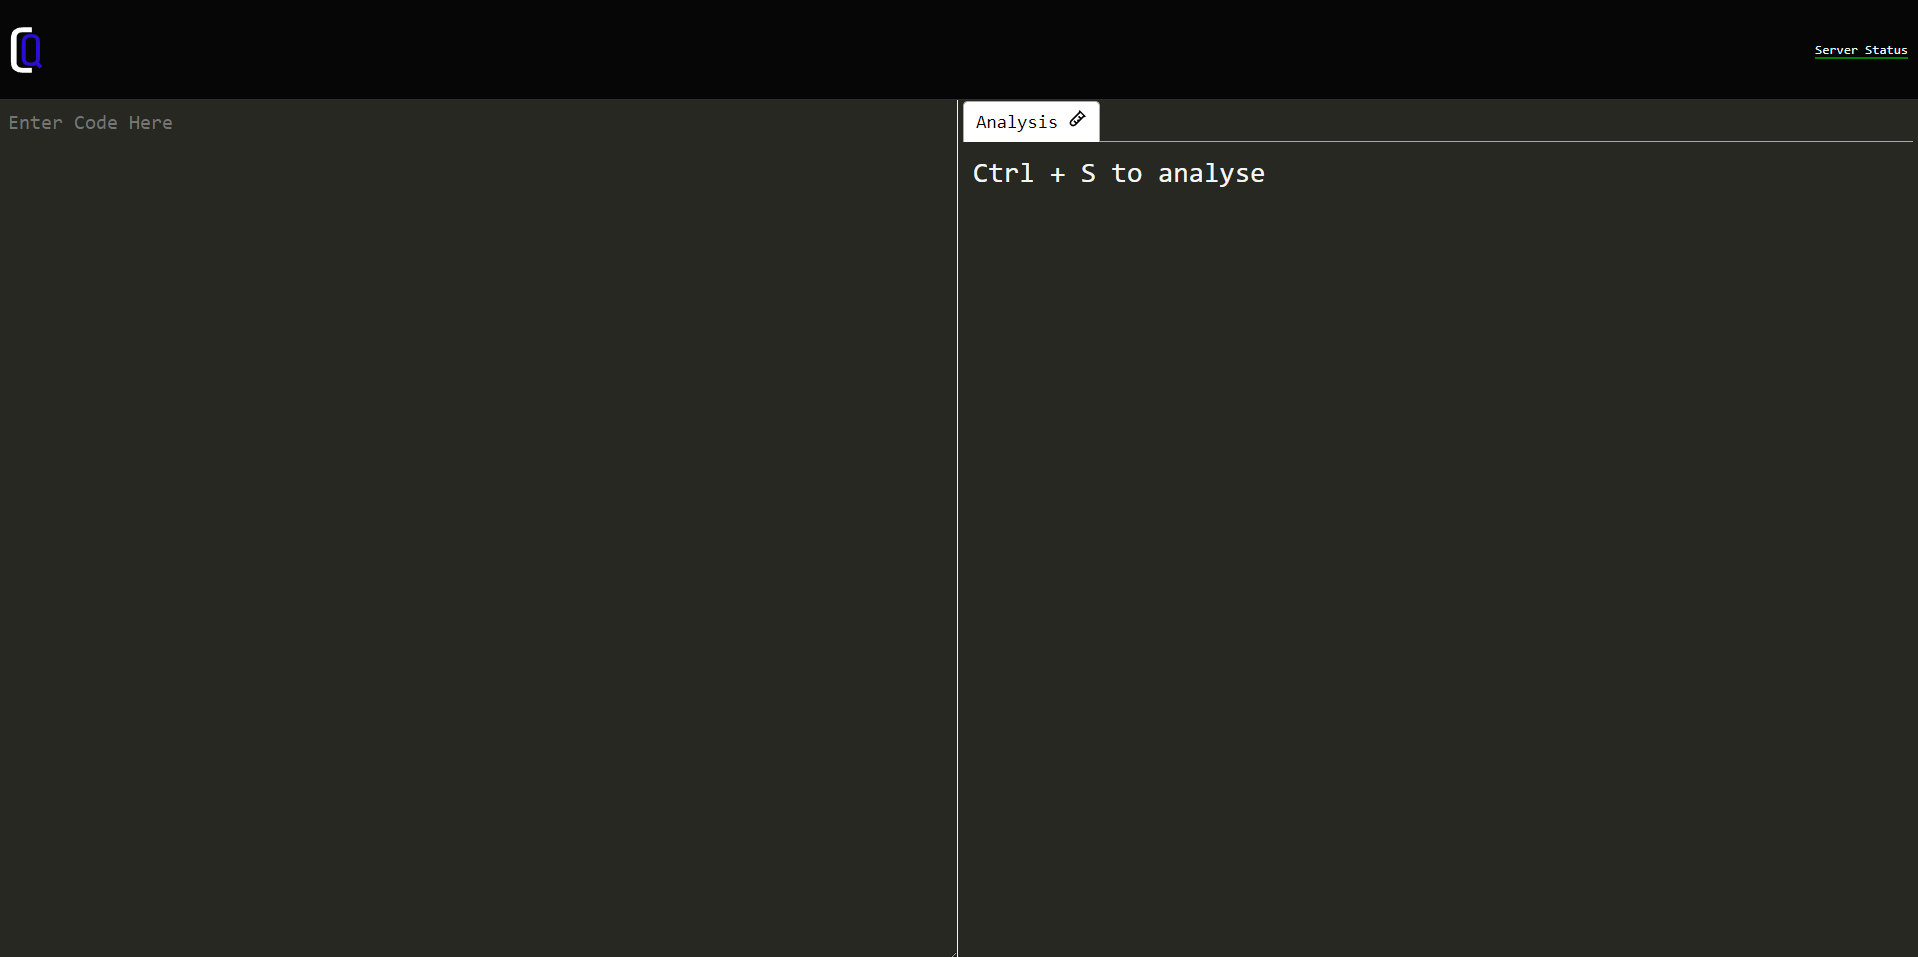
\includegraphics[width=.5\textwidth]{images/final-screenshot.png}
    \caption{Final Product See Appendix U}
    \Description{Final Product See Appendix U}
    \label{fig:finalproduct}
\end{figure}
\newline
\newline
\textbf{Code Editor}
\newline
In Figure \RefFig{fig:autocomplete} we can see a screenshot of the autocomplete feature, this allows the user to autocomplete code using a list of all 
the javascript reserved words and any words already typed in the editor by pressing tab
\newline
The user will also have brackets and strings autofilled while typing.
\begin{figure}[h]
    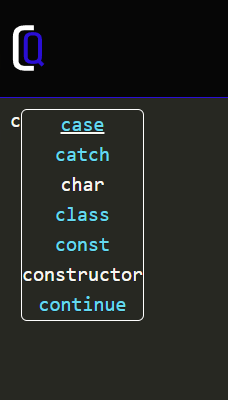
\includegraphics[width=.3\textwidth]{images/autocomplete.png}
    \caption{AutoComplete See Appendix U}
    \Description{AutoComplete See Appendix U}
    \label{fig:autocomplete}
\end{figure}
In Figure \RefFig{fig:Highliting} we can see the code the user has entered that has been highlighted.
\begin{figure}[h]
    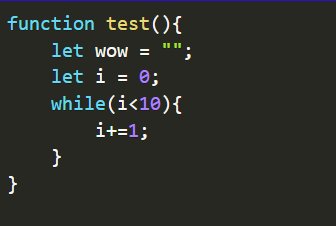
\includegraphics[width=.3\textwidth]{images/Highlighted.png}
    \caption{Highlighted Source Code See Appendix U}
    \Description{Highlighted Source Code See Appendix U}
    \label{fig:Highliting}
\end{figure}
\newline
\newline
\textbf{Analysis}
\newline
In Figure \RefFig{fig:output} we can see the output in the analysis panel, this displays the output of the analysis on the code alongside the 
source code. Also in Figure \RefFig{fig:clickfunc} we can see that clicking on a element in the output panel highlights that code within the code editor. Finally in Figure \
The download button shown in \RefFig{fig:downloadbutton} allows the user to download a copy of the report.
\newline
In Figure \RefFig{fig:astpanel} we can see the ast panel which allows users to view the AST of their source code.
\begin{figure}[h]
    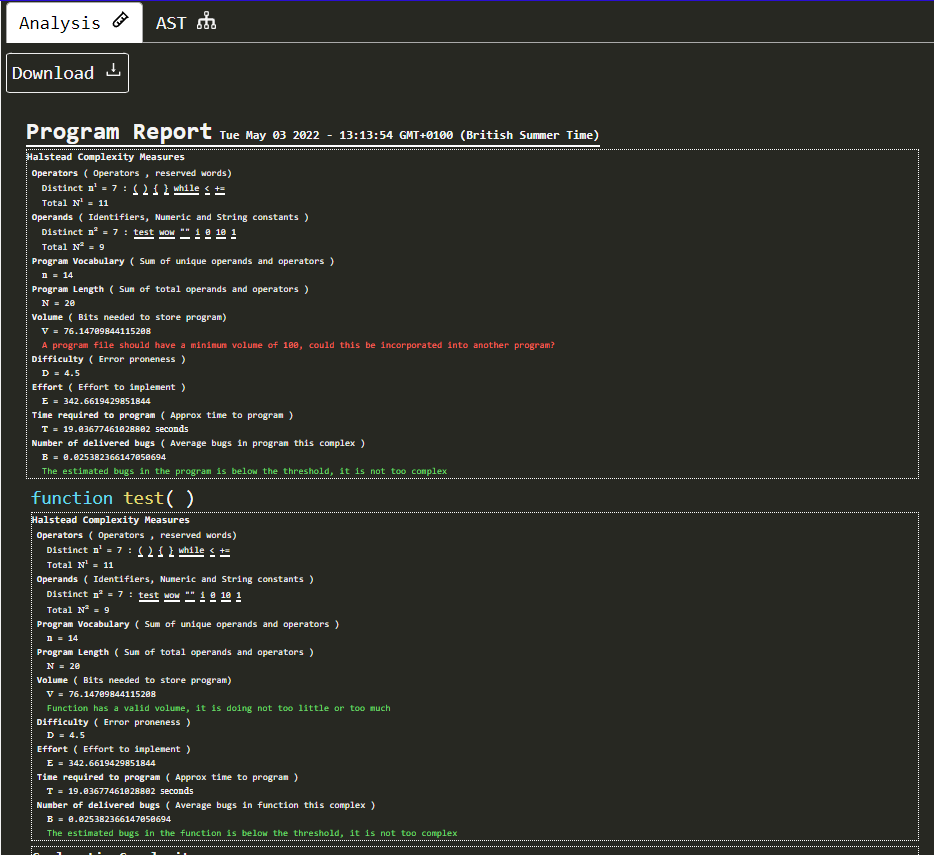
\includegraphics[width=.5\textwidth]{images/analysisoutput.png}
    \caption{Analysis Output See Appendix U}
    \Description{Analysis Output See Appendix U}
    \label{fig:output}
\end{figure}

\begin{figure}[h]
    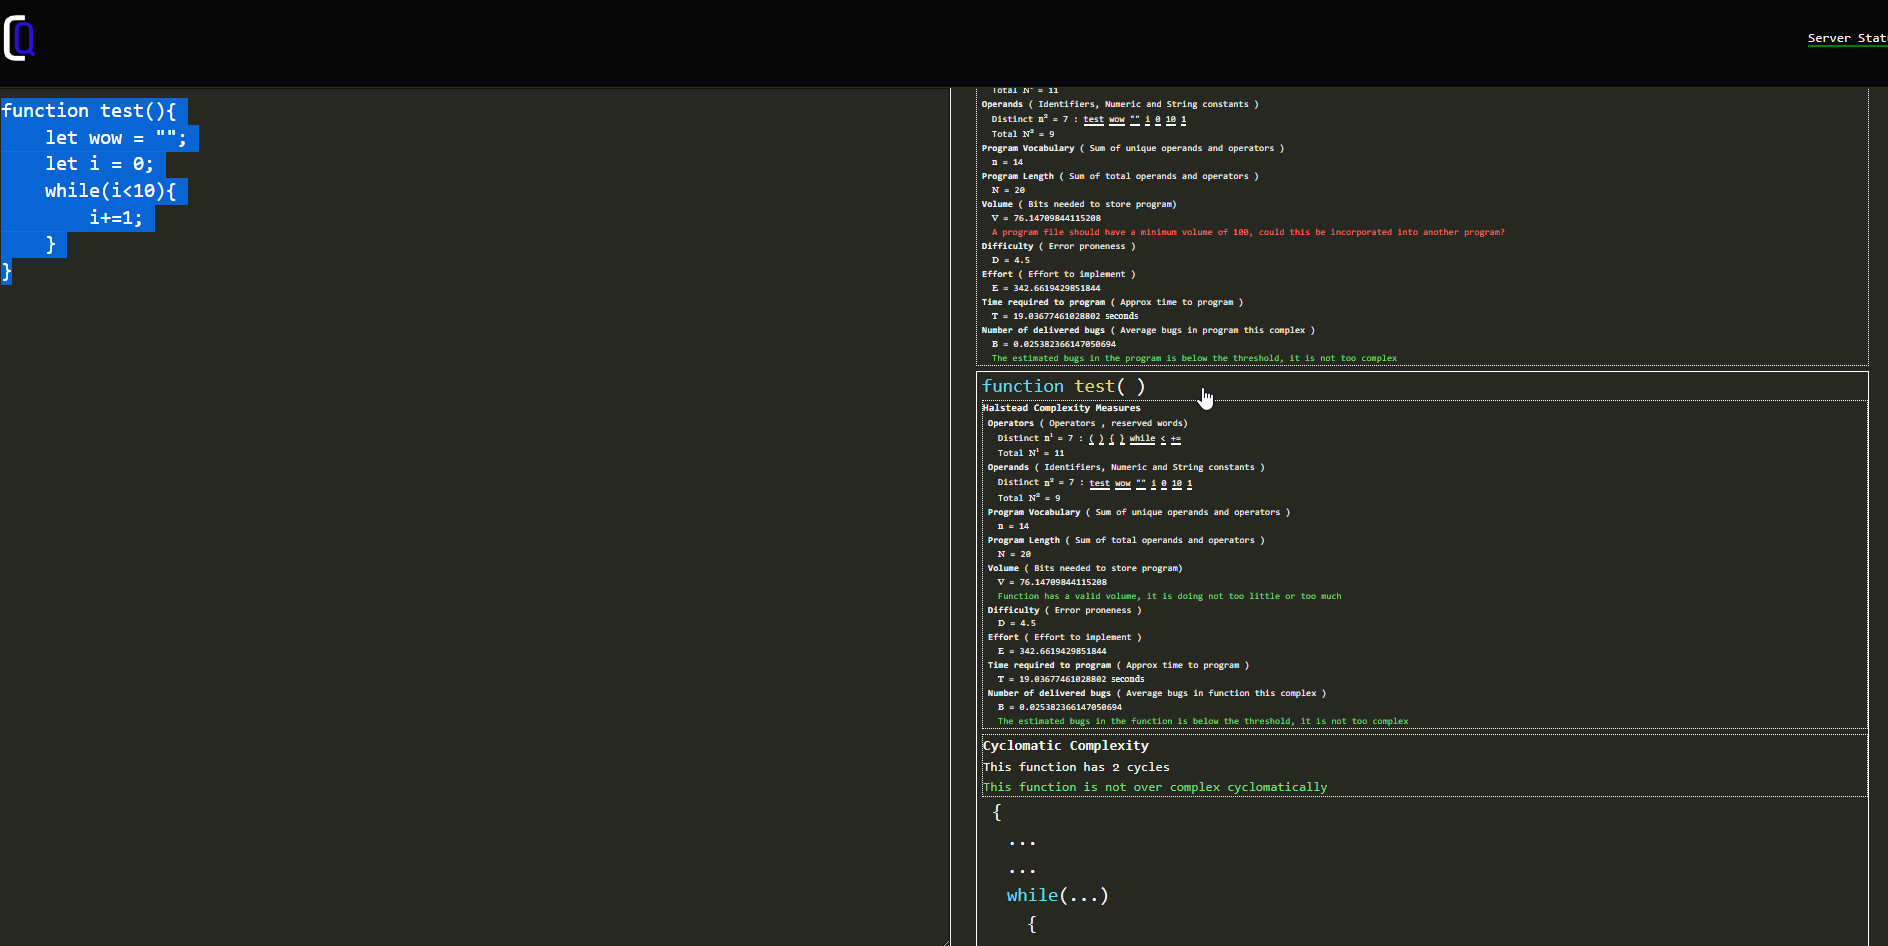
\includegraphics[width=.5\textwidth]{images/clickfunc.png}
    \caption{Clicking on function in analysis See Appendix U}
    \Description{Clicking on function in analysis See Appendix U}
    \label{fig:clickfunc}
\end{figure}
\begin{figure}[h]
    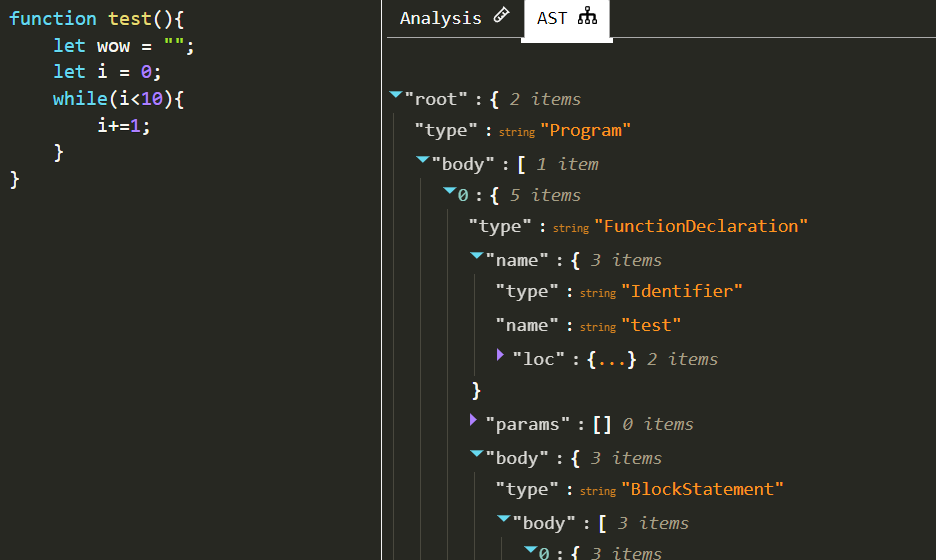
\includegraphics[width=.5\textwidth]{images/ast.png}
    \caption{AST panel See Appendix U}
    \Description{AST panel See Appendix U}
    \label{fig:astpanel}
\end{figure}
\begin{figure}[h]
    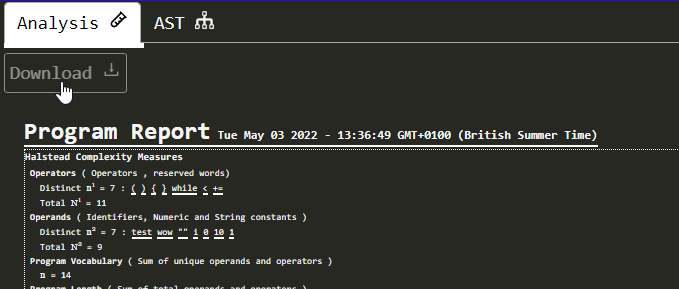
\includegraphics[width=.4\textwidth]{images/downloadbutton.png}
    \caption{Download Button See Appendix U}
    \Description{Download Button See Appendix U}
    \label{fig:downloadbutton}
\end{figure}

In figure \RefFig{fig:syntax1} we can see that the user has entered incorrect syntax. By then opening the syntax panel and clicking on the error , 
the user can find the syntax error in the code, as shown in Figure \RefFig{fig:syntax2}
\begin{figure}[h]
    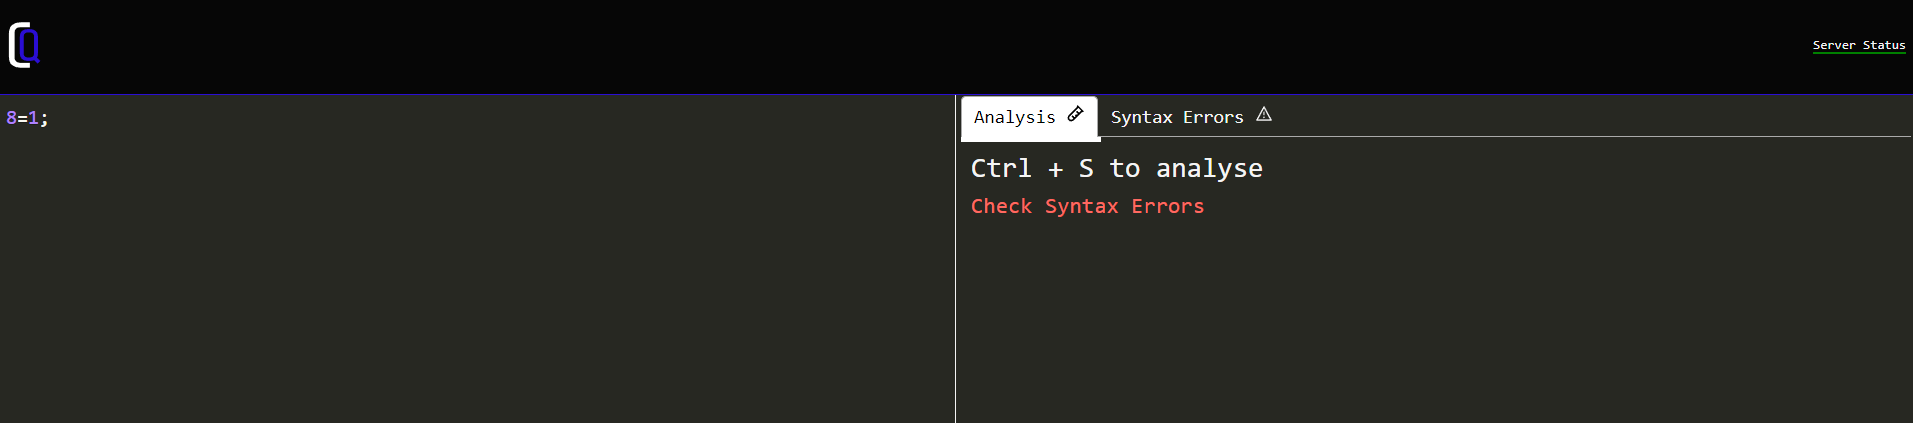
\includegraphics[width=.5\textwidth]{images/syntax1.png}
    \caption{Syntax Error See Appendix U}
    \Description{Syntax Error See Appendix U}
    \label{fig:syntax1}
\end{figure}
\begin{figure}[h]
    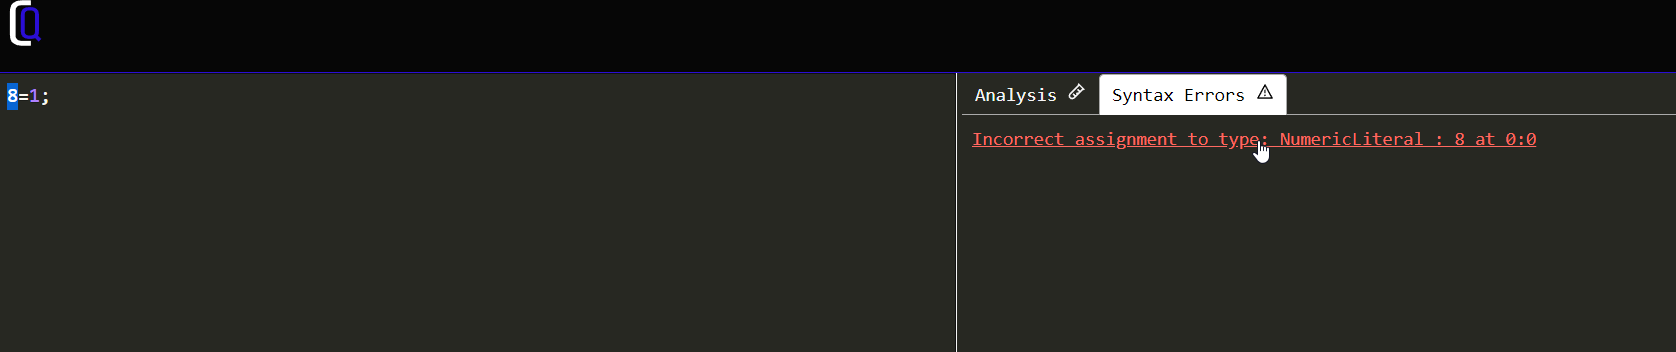
\includegraphics[width=.5\textwidth]{images/syntax2.png}
    \caption{Syntax Error Clicking See Appendix U}
    \Description{Syntax Error Clicking See Appendix U}
    \label{fig:syntax2}
\end{figure}
\newpage
\section{Appraisal}

\section{Conclusion}
The goal of this project was to understand the code quality analysis process and 
learn how parsing is done, the student believes this has been achieved. The artifact produced 
meets the requirements of 18/30 of the user stories created, with the majority of the stories left 
uncompleted being smaller stories that are made easier by the work that has been completed.
\newline
Coming into this project with no understanding of how static analysis worked and how parsers were 
made it has been a great learning experience that the student believes will benefit them 
in the long term.
how do we take what we have learned forward 
\newline
The final artifact created needs work to be a widely used application but as the results from the 
user testing show, it has created an interest in the participants in code quality analysis. This is justification 
enough to the student that it has been a success.
\section{Future Work}
\begin{figure}
    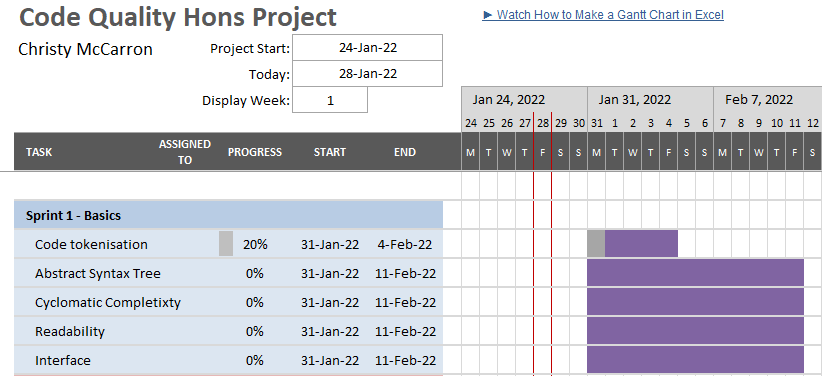
\includegraphics[width=.2\textwidth]{images/gantt.png}
    \caption{Gantt Sprint 1}
    \Description{gantt for sprint 1}
    \label{fig:gantt}
  \end{figure}
  Reflecting on the progress so far I believe that I have done a good amount of research which I will now apply to coding, I wish I had started prototying earlier as that would have made the planning much easier to estimate time.
  \newline
  As I am following agile I have made simple plans for sprint 1 where my sprints will be 2 weeks, after the end of sprint I will have a retrospective and review the progress completed in sprint 1.
  \newline
  I believe over the course of the project I should be able to complete every user story following this model.
  \newline
  The biggest pitfall that should be encountered is ensuring the abstract syntax tree is correct is this is the bed that everything else lies on, to ensure this it will be developed with a massive amount of unit and integration testing.


  javscript full syntax

  allow settings 

  cyclomatic complexity extended to logical statements 





%%
%% The acknowledgments section is defined using the "acks" environment
%% (and NOT an unnumbered section). This ensures the proper
%% identification of the section in the article metadata, and the
%% consistent spelling of the heading.
\begin{acks}
The author wishes to thank their advisor Dr. Craig Ramsay for their help through the entire process, who was always prompt with communication and willing to set up meetings right until the very end. Furthermore was willing to bounce ideas off constantly.
\newline
\newline
The author would like to thank Dr. Michael Crabb the Teaching Lead for computing at University of Dundee, for the creation of the LaTeX template which was used to write this report.
\newline
\newline
The author would like to bring attention to the writings of 
Aaron Swartz on \href{https://archive.org/stream/GuerillaOpenAccessManifesto/Goamjuly2008_djvu.txt}{\underline{The Guerilla Open Access Manifesto}} , without the principles therein it would have been much more difficult to complete the project.

\end{acks}

%%
%% The next two lines define the bibliography style to be used, and
%% the bibliography file.
\bibliographystyle{ACM-Reference-Format}
\bibliography{references}

%%
%% If your work has an appendix, this is the place to put it.
\appendix

\huge{\textbf{Appendices}}
\newline
\normalsize{Each appendix can be found either as a \underline{LINK} or in the sub folder with it's label, e.g. Appendix A is found in the path "/A/"}
\section{Control Flow Graph}
\section{Code Analyser Diagram}
\section{Compiler Diagram}
\section{User Personas}
\section{User Stories}
\section{Github Issues}
\url{https://github.com/aliveSurfin/code_quality/issues}
\section{MoSCoW Analysis}
\url{https://github.com/aliveSurfin/code_quality/projects/1}
\section{Value Risk}
\url{https://github.com/aliveSurfin/code_quality/projects/2}
\section{Combined MoscowValueRisk Priorities}
\url{https://github.com/aliveSurfin/code_quality/projects/3}
\section{T-Shirt Sizing}
\url{https://github.com/aliveSurfin/code_quality/projects/4}
\section{Source Code}
\url{https://github.com/aliveSurfin/code_quality/blob/main/development/code}
\section{Left Most Derivation Diagram}
\section{Right Most Derivation Diagram}
\section{Code Editor Initial Designs}
\section{Parser}
\url{https://github.com/aliveSurfin/code_quality/blob/main/development/code/parsing/parser/Parser.js}
\section{AST Types}
\url{https://github.com/aliveSurfin/code_quality/blob/main/development/code/parsing/parser/AST_CONST_TYPES.js}
\section{Tokeniser Folder}
\url{https://github.com/aliveSurfin/code_quality/tree/main/development/code/parsing/tokenizer}
\section{Parser Tests}
\url{https://github.com/aliveSurfin/code_quality/tree/main/development/code/parsing/parser/tests}
\section{Development Diary}
\url{https://github.com/aliveSurfin/code_quality/blob/main/development/diary/diary.md}
\section{Evaluation Features}
\url{https://github.com/aliveSurfin/code_quality/tree/main/development/code/parsing/evaluate}
\section{Final Product}
\url{https://code-quality-honours.herokuapp.com/}
\section{Code Coverage}
\section{Interview Notes}
\section{User Testing Results}


\end{document}
\endinput
%%
%% End of file `sample-sigconf.tex'.
